\documentclass[border=10pt]{standalone}

\usepackage{tikz}
\usepackage{tikzsymbols}
\usetikzlibrary{calc,patterns,shapes.geometric}

\def\centerarc[#1](#2)(#3:#4:#5){\draw[#1] ($(#2)+({#5*cos(#3)},{#5*sin(#3)})$) arc (#3:#4:#5);}

\begin{document}
	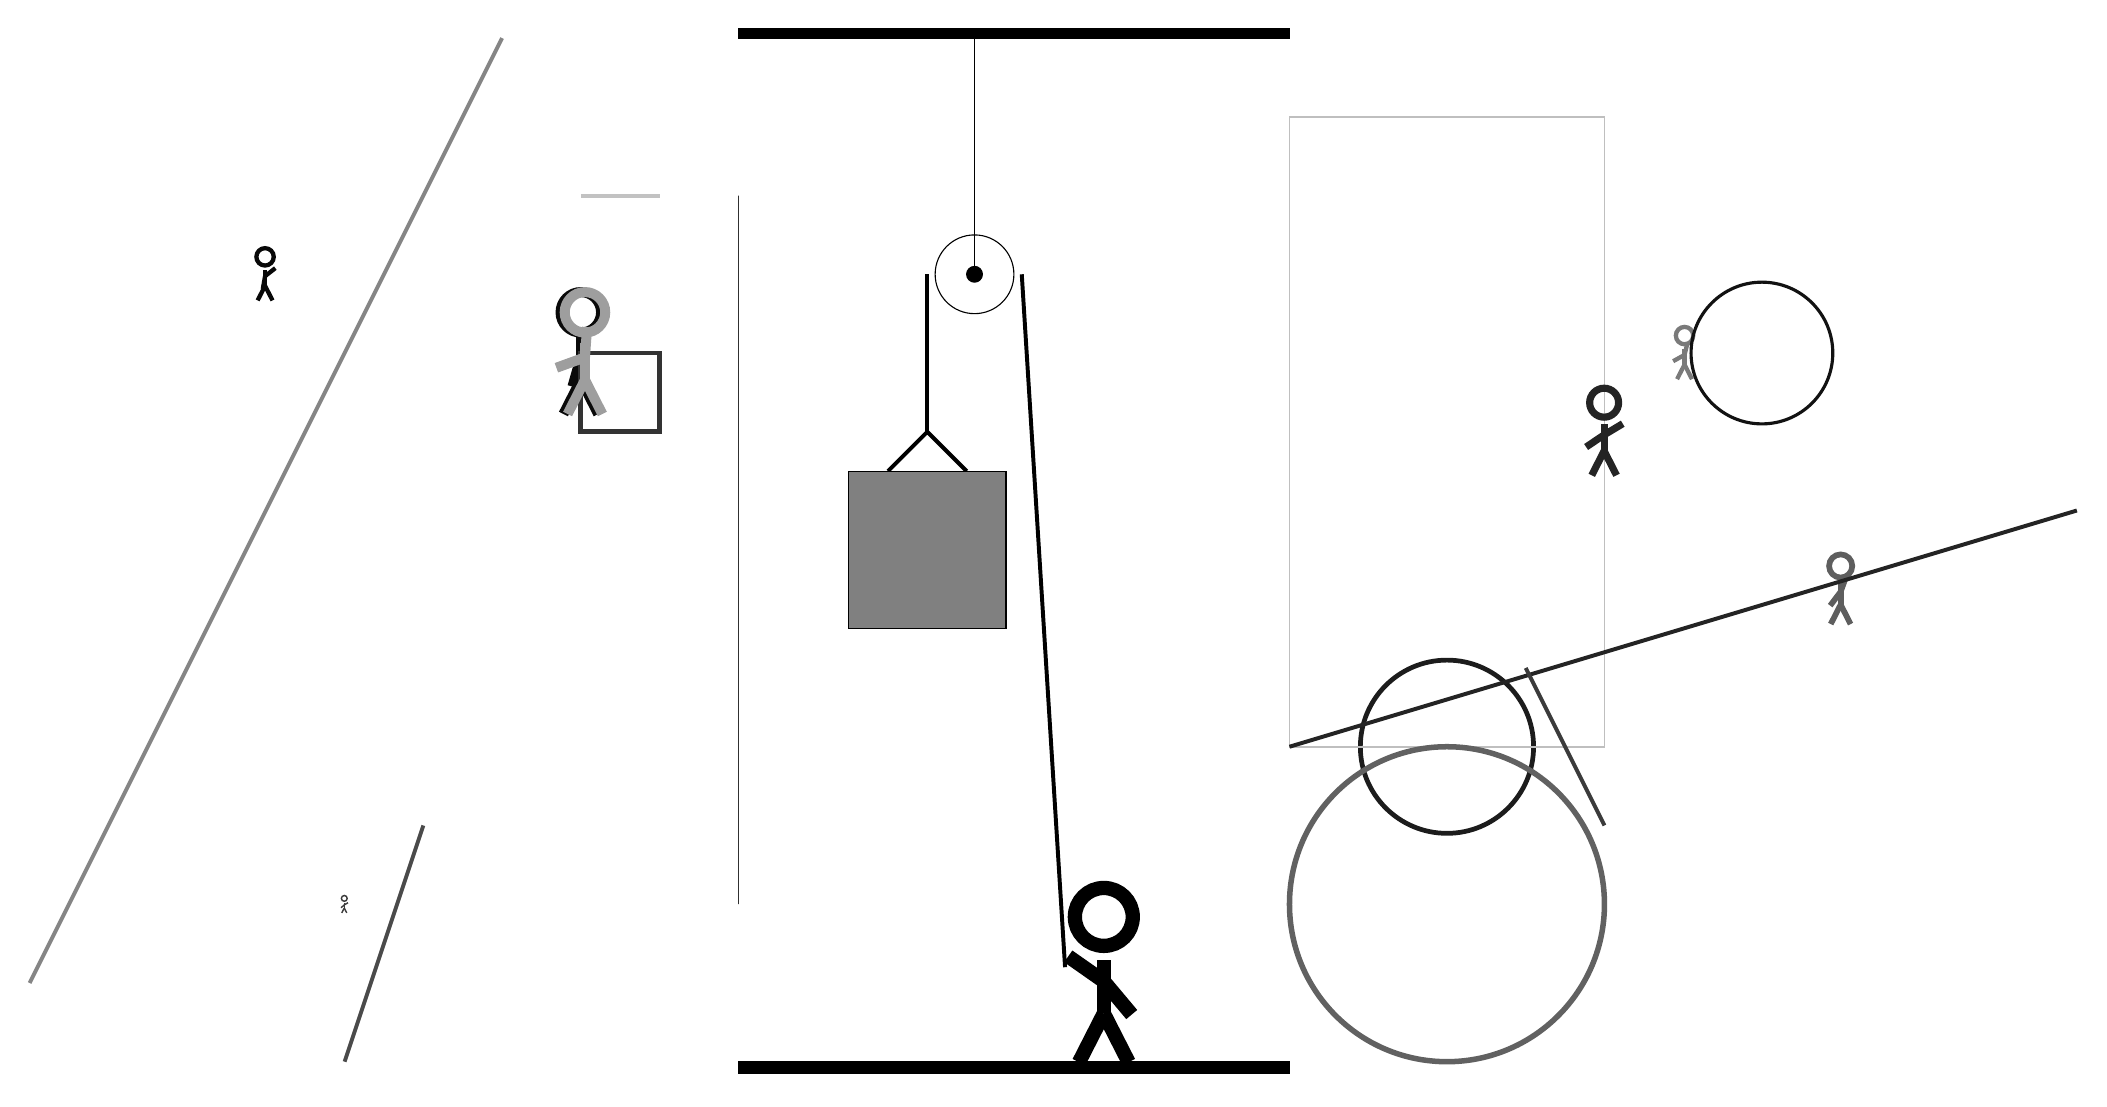
\begin{tikzpicture}
		%%%%% START %%%%%
		
		\draw[fill=black] (-2, 10) rectangle (5, 10.125);
		
		\draw (1, 7) circle (0.5);
		\draw[fill=black] (1, 7) circle (0.1);
		\draw (1, 10) -- (1, 7);
		
		\draw[line width=0.5mm] (-0.1, 4.5) -- (0.4, 5.0) -- (0.9, 4.5);
		\draw[fill=black!50] (-0.6, 4.5) rectangle (1.4, 2.5);
		
		\draw[line width=0.5mm] (0.4, 7) -- (0.4, 5.0);
		\centerarc[line width=0.5mm](1, 7)(0:180:0.6);
		\draw[line width=0.5mm](1.6, 7) -- (2.15, -1.8);
		
		\node at (2.6, -1.9) {\Strichmaxerl[10][-35][-50]};
		
		\draw [line width=0.6mm, color=black!89](7, 1) circle (1.1);
		
		\draw[line width=0.5mm, color=black!48](-5, 10) -- (-11, -2);
		\draw[line width=0.5mm, color=black!70](5, -1) -- (5, -1);
		\draw[line width=0.2mm, color=black!25] (5, 9) rectangle (9, 1);
		
		\node[line width=0.4mm, color=black!96] at (-4, 6) {\Strichmaxerl[7][74][90]};
		\node[line width=0.7mm, color=black!63] at (12, 3) {\Strichmaxerl[4][53][70]};
		
		\node[line width=0.6mm, color=black!52] at (10, 6) {\Strichmaxerl[3][29][76]};
		
		\draw[line width=0.5mm, color=black!71](-7, -3) -- (-6, 0);
		\draw[line width=0.5mm, color=black!86](5, 1) -- (15, 4);
		
		\draw [line width=0.4mm, color=black!93](11, 6) circle (0.9);
		
		\draw[line width=0.6mm, color=black!80] (-3, 6) rectangle (-4, 5);
		\draw [line width=0.7mm, color=black!62](7, -1) circle (2.0);
		\draw[line width=0.5mm, color=black!24](-4, 8) -- (-3, 8);
		
		\node[line width=0.2mm, color=black!97] at (-8, 7) {\Strichmaxerl[3][80][38]};
		\node[line width=0.6mm, color=black!77] at (-7, -1) {\Strichmaxerl[1][43][29]};
		\node[line width=0.3mm, color=black!38] at (-4, 6) {\Strichmaxerl[7][20][86]};
		
		\draw[line width=0.5mm, color=black!77](8, 2) -- (9, 0);
		\node[line width=0.7mm, color=black!86] at (9, 5) {\Strichmaxerl[5][34][31]};
		\draw[line width=0.2mm, color=black!81] (-2, -1) rectangle (-2, 8);
		
		
		\draw[fill=black] (-2, -3) rectangle (5, -3.15);
		
		%%%%% END %%%%%
	\end{tikzpicture}
\end{document}